\section{Experiments}
\label{sec:exp}

Section~\ref{sec:expset} details the test corpus to be induced and
experiment parameters used in the rest of this work.

%% The S-CODE algorithm (Section~\ref{sec:codethr}) works with discrete
%% inputs.  The substitute vectors as described in
%% Section~\ref{sec:subcomp} are high dimensional and continuous.
%% Section~\ref{sec:wordsub-type} introduces a simple method to
%% discretize the substitute vectors by randomly sampling from the
%% distributions for the POS induction of the word types.
%% Section~\ref{sec:wordsub-token} leverages the same random sampling
%% idea and applies it to the POS induction of word tokens by adding a
%% post--processing step to the output of the S-CODE algorithm.

Section~\ref{sec:bigram-type} and Section~\ref{sec:bigram-token} aim
to compare our paradigmatic representation of the word context to
previously described syntagmatic representations of the word context
for word types and word tokens, respectively.
Section~\ref{sec:bigram-type} also replicates the bigram based S-CODE
results from \cite{maron2010sphere}.

Section~\ref{sec:feat} explores morphological and orthographic
features as additional sources of information for POS induction of
word types and its results improve the state-of-the-art in the field
of POS induction.

\subsection{Experimental Settings}\label{sec:expset}

To make a meaningful comparison to the previous works
% what is the test data
the Wall Street Journal Section of the Penn Treebank (PTB) \cite{treebank3}
was used as the test corpus (1,173,766 tokens, 49,206 types) to be
induced.
% what is the tag set
The treebank uses 45 part-of-speech tags which is the set we used as
the gold standard for comparison in our experiments.

% what is the LM training data
%Train => 5181717 126019973 690121813
To compute substitutes in a given context we trained a language model
using approximately 126 million tokens of Wall Street Journal data
(1987-1994) extracted from CSR-III Text \cite{csr3text} (excluding
sections of the PTB).
% how is the language model trained
We used SRILM \cite{Stolcke2002} to build a 4-gram language model with
Kneser-Ney discounting.
% what is the vocabulary
Words that were observed less than 20 times in the language model
training data were replaced by \textsc{unk} tags, which gave us a
vocabulary size of 78,498.
% what is the test data
% perplexity
The perplexity of the 4-gram language model on the test corpus is 96.
For computational efficiency only the top 100 substitutes and their
unnormalized probabilities were computed for each positions in the PTB
% (1,173,766 tokens, 49,206 types)
using the {\sc fastsubs} algorithm
\cite{yuret2012fastsub}\footnote{The substitutes with unnormalized log
  probabilities can be downloaded from
  \mbox{\url{http://goo.gl/jzKH0}}.}.  The probability vectors for
each position were normalized to add up to 1.0 giving us the final
substitute distributions used in the rest of this study.

% To make a meaningful comparison on the PTB
The experiments were run using the following default settings (unless
otherwise stated): (i) each word was kept with its original
capitalization, (ii) the learning rate parameters were set to
$\varphi_0=50$, $\eta_0=0.2$ for faster convergence in log likelihood,
(iii) the number of S-CODE iterations were set to 50 million, (iv) the
S-CODE dimensions and $Z$ were set to 25 and 0.166, respectively, (v)
a modified k-means algorithm with smart initialization was used
\cite{arthur2007k}, and (vi) the number of k-means restarts were set
to 128 to improve clustering and reduce variance.

Each experiment was repeated 10 times with different random seeds and
the results are reported with standard errors in parentheses or error
bars in graphs.  Table~\ref{tab:results} summarizes all the results
reported in this section and the ones we cite from the literature.

\subsection{Clustering Word Embeddings ({\bf W})}
\label{sec:wordsub-type}

The S-CODE uses stochastic gradient ascent (see
Appendix~\ref{sec:codethr}) to find the $\phi_w, \psi_s$ embeddings
for word and random-substitute in these pairs on a single
25-dimensional sphere.  The algorithm cycles through the data until we
get approximately 50 million updates.  The resulting $\phi_w$ vectors
are clustered using an instance weighted k-means algorithm.
Cluster-id for each $\phi_w$ is assigned as the predicted cluster-id
for word type $W$.  Using the default settings and sampling 64
substitutes for each token the many-to-one accuracy is \wsmto and the
V-measure is \wsvm.

\begin{table*}[t] \footnotesize
\caption{Summary of results in terms of the \mto\ and \vm\ scores.
  Standard errors are given in parentheses when available.  Starred
  entries have been reported in the review paper
  \protect\cite{Christodoulopoulos:2010:TDU:1870658.1870714}.  Distributional
  models use only the identity of the target word and its context.
  The models on the right incorporate orthographic and
  morphological features.}
\begin{tabular}{|@{ }l@{ }|@{ }l@{ }|@{ }l@{ }|}
\hline
Distributional Models & \mto & \vm \\
\hline
Lamar et al. \shortcite{Lamar:2010:LCU:1870658.1870736} & .708 & -\\ %algorithm name LDC
Brown et al. \shortcite{Brown:1992:CNG:176313.176316}* & .678 & .630\\
%kcls(Och,1999) & .737 & .656\\
%\cite{goldwater-griffiths:2007:ACLMain} & .632 & .562\\
Goldwater et al. \shortcite{goldwater-griffiths:2007:ACLMain}* & .632 & .562\\
Ganchev et al. \shortcite{Ganchev:2010:PRS:1859890.1859918}* & .625 & .548\\
Maron et al. \shortcite{maron2010sphere} & .688 (.0016)&-\\
Substitutes(Tokens) (Sec.~\ref{sec:tokens}) & \wsxymto & \wsxyvm \\
Bigrams (Sec.~\ref{sec:bigram}) & \bgmto & \bgvm \\
%Partitions (Sec.~\ref{sec:rpart}) & \rpmto & \rpvm \\
Substitutes(Types) (Sec.~\ref{sec:wordsub}) & \wsmto & \wsvm \\
\hline
\end{tabular}
\begin{tabular}{|@{ }l@{ }|@{ }l@{ }|@{ }l@{ }|}
\hline
Models with Additional Features & \mto & \vm \\
\hline
Clark \shortcite{Clark:2003:CDM:1067807.1067817}* & .712 & .655 \\
Christodoulopoulos et al. \shortcite{christodoulopoulos-goldwater-steedman:2011:EMNLP} & .728 & .661\\
Berg-Kirkpatrick et al. \shortcite{bergkirkpatrick-klein:2010:ACL} & .755 & -\\ % Interesting in  christo paper:73.9/67.7
Christodoulopoulos et al. \shortcite{Christodoulopoulos:2010:TDU:1870658.1870714} & .761 & .688\\
Blunsom and Cohn \shortcite{blunsom-cohn:2011:ACL-HLT2011} & .775 & .697\\
Substitutes and Features (Sec.~\ref{sec:feat}) & \ftmto & \ftvm \\
& & \\
& & \\
\hline
\end{tabular}
\label{tab:results}
\end{table*}

%% Moved to appendix
%% To obtain a discrete representation of the context, the
%% random-substitutes algorithm pairs each word token with a substitute
%% sampled from the pre-computed substitute vectors generated from the
%% word token's context (see Section~\ref{sec:subcomp}) and word ($X$) --
%% random-substitute ($Y$) pairs are fed to the S-CODE as input.  It is
%% possible (and beneficial, see below) to run the random-substitutes
%% algorithm on the data more than once to generate more pairs from the
%% same substitute vectors. 

%% To obtain a discrete representation of the context, the
%% random--partitions algorithm first designates a random subset of
%% substitute vectors as centroids to partition the space, and then
%% associates each context with the partition defined by the closest
%% centroid in cosine distance.  Each partition thus defined gets a
%% unique id, and word ($X$) -- partition-id ($Y$) pairs are given to
%% S-CODE as input.  The algorithm uses stochastic gradient ascent to
%% find the $\phi_x, \psi_y$ embeddings for word and partition-id in
%% these pairs on a single 25-dimensional sphere.  The algorithm cycles
%% through the data until we get approximately 50 million updates.  The
%% resulting $\phi_x$ vectors are clustered using an instance weighted
%% k-means algorithm and the resulting groups are compared to the correct
%% part of speech tags.  Using default settings with 64K random
%% partitions the many-to-one accuracy is \rpmto\ and the V-measure is
%% \rpvm.

To analyze the sensitivity of this result to our specific parameter
settings we ran a number of experiments where each parameter was
varied over a range of values.

%% \begin{figure}[ht] \centering
%% 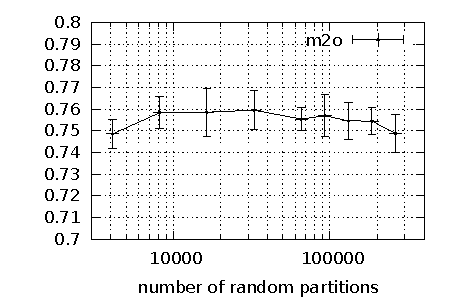
\includegraphics[width=0.5\linewidth]{plot-p.pdf}
%% \caption{\mto\ is not sensitive to the number of partitions used to
%%   discretize the substitute vector space within our experimental
%%   range.}
%% \label{plot-p}
%% \end{figure}

%% Figure~\ref{plot-p} gives results where the number of initial random
%% partitions is varied over a large range and shows the results to be
%% fairly stable across two orders of magnitude.

\begin{figure}[ht] \centering
%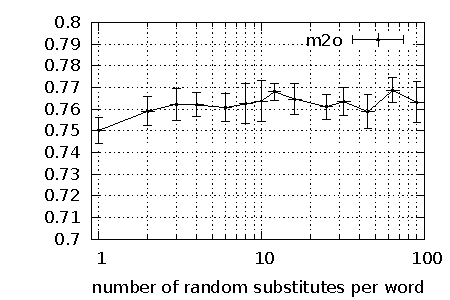
\includegraphics[width=0.5\linewidth]{plot-s.pdf}
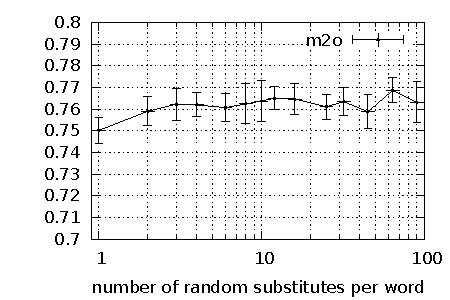
\includegraphics[width=0.5\linewidth]{plot-s-cl.pdf}
\caption{\mto\ is not sensitive to the number of random substitutes
  sampled per word token.}
\label{plot-s}
\end{figure}

Figure~\ref{plot-s} illustrates that the
random-substitute result is fairly robust as long as the training
algorithm can observe more than a few random substitutes per word.

\begin{figure}[ht] \centering
%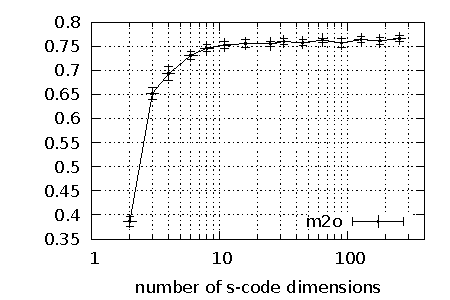
\includegraphics[width=0.5\linewidth]{plot-d.pdf}
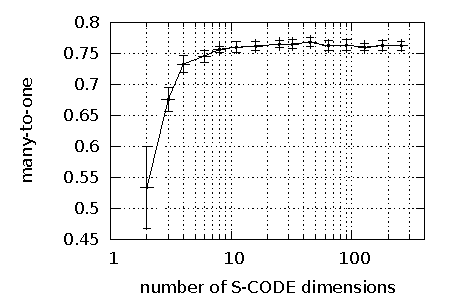
\includegraphics[width=0.5\linewidth]{plot-d-cl.pdf}
\caption{\mto\ falls sharply for less than 10 S-CODE dimensions, but
  more than 25 do not help.}
\label{plot-d}
\end{figure}

Figure~\ref{plot-d} shows that at least 10 embedding dimensions are
necessary to get within 1\% of the best result, but there is no
significant gain from using more than 25 dimensions.

\begin{figure}[ht] \centering
%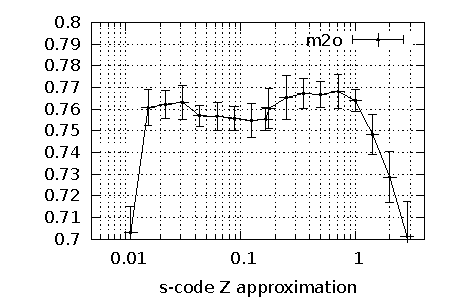
\includegraphics[width=0.5\linewidth]{plot-z.pdf}
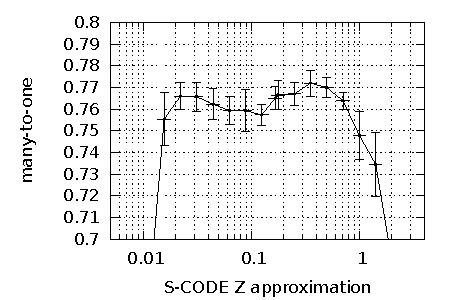
\includegraphics[width=0.5\linewidth]{plot-z-cl.pdf}
\caption{\mto\ is fairly stable as long as the $\tilde{Z}$ constant is
  within an order of magnitude of the real $Z$ value.}
\label{plot-z}
\end{figure}

Figure~\ref{plot-z} shows that the constant $\tilde{Z}$ approximation
can be varied within two orders of magnitude without a significant
performance drop in the many-to-one score.  For uniformly distributed
points on a 25 dimensional sphere, the expected $Z\approx 0.146$.  In
the experiments where we tested we found the real $Z$ always to be in
the 0.140-0.170 range.  When the constant $\tilde{Z}$ estimate is too
small the attraction in Eq.~\ref{eq:attract} dominates the repulsion
in Eq.~\ref{eq:repulse} and all points tend to converge to the same
location.  When $\tilde{Z}$ is too high, it prevents meaningful
clusters from coalescing.
%%% I have seen the first, but the second is pure guess, need to
%%% look.  The distances seem to be decreasing on that end as well!

We find our model with random substitute to be fairly robust to
different parameter settings and the resulting many-to-one score
significantly better than the state-of-the-art distributional models.

%% We find the random partition algorithm to be fairly robust to
%% different parameter settings and the resulting many-to-one score
%% significantly better than the state-of-the-art distributional models.

%% \subsection{Random Substitutes}\label{sec:wordsub}

%% Another way to use substitute vectors in a discrete setting is simply
%% to sample individual substitute words from them according to the
%% corresponding probabilities.  The random-substitutes algorithm cycles
%% through the test data and pairs each word with a random substitute
%% picked from the pre-computed substitute vectors (see
%% Section~\ref{sec:subthr}).  We ran the random-substitutes algorithm to
%% generate 76 million word ($X$) -- random-substitute ($Y$) pairs (64
%% substitutes for each token) as input to S-CODE.  Clustering the
%% resulting $\phi_x$ vectors yields a many-to-one score of \wsmto\ and a
%% V-measure of \wsvm.

%% This result is close to the previous result by the random-partition
%% algorithm, \rpmto, demonstrating that two very different discrete
%% representations of context based on paradigmatic features give
%% consistent results.  Figure~\ref{plot-s} illustrates that the
%% random-substitute result is fairly robust as long as the training
%% algorithm can observe more than a few random substitutes per word.

%% \begin{figure}[ht] \centering
%% 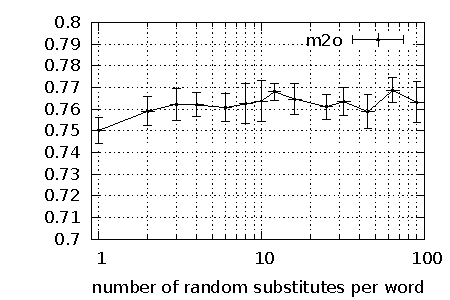
\includegraphics[width=0.5\linewidth]{plot-s.pdf}
%% \caption{\mto\ is not sensitive to the number of random substitutes
%%   sampled per word token.}
%% \label{plot-s}
%% \end{figure}

\subsection{Paradigmatic vs Syntagmatic Representations of Word Context}
\label{sec:bigram-type}

To get a direct comparison of the paradigmatic and syntagmatic context
representations we feed 4 different co-occurrences defined in
Section~\ref{sec:representation} into the S-CODE algorithm.  The first
model accepts word ($X$) - right bigram ($Y$) pairs as the input, the
second model accepts word ($X$) - left bigram($Y$) pairs as the input,
the third model accepts word ($X$) - concatenation of the left and
right bigrams ($Y$) pairs \cite{mintz2003frequent} as the input and
the final model accepts words ($X$) - left bigram($Y_1$) and right
bigram ($Y_2$) tuples \cite{20674613} as the input to the S-CODE.  At
the end we cluster the word types ($X$) with k-means algorithm and
report the results on Table \ref{tab:syntagmatic}.

\begin{table}[ht]
\caption{Summary of results in terms of the \mto\ and \vm\ scores of
  the S-CODE algorithm when the paradigmatic or syntagmatic
  representations are feed as an input.  Standard errors are given in
  parentheses when available.  Results of the statistically best
  performing system are written in bold.  We do not report the
  original results of Maron et al. \protect\shortcite{maron2010sphere}
  since our replication achieves higher accuracies.}
\begin{tabular}{|l|l|l|}
\hline
Input & \mto & \vm\\
\hline
$X$ (word) - $Y$ (right bigram) & .6625 (.0115) & .5809 (.0066)\\
$X$ (word) - $Y$ (left bigram) & .6604 (.0054) & .5983 (.0028)\\
$X$ (word) - $Y$ (left and right bigram concatenation) & .7268 (.0091) & .6416 (.0052)\\
$X$ (word) - $Y_1$, $Y_2$ (left and right bigrams) & .7173 (.0061) & .6381 (.0032)\\
Maron et al. \shortcite{maron2010sphere}(replication)  & \bgmto & \bgvm \\
$X$ (word) - $Y$ (random substitutes) & {\bf\wsmto} & {\bf\wsvm} \\
\hline

\hline
\end{tabular}
\label{tab:syntagmatic}
\end{table}

To replicate the work of Maron et al. \shortcite{maron2010sphere} we
feed word ($X$) - right bigram ($Y$) pairs as the input.  At the end
each word $w$ in the vocabulary ends up with two points on the sphere,
a $\phi_w$ point representing the behavior of $w$ as the left word of
a bigram and a $\psi_w$ point representing it as the right word.  The
two vectors for $w$ are concatenated to create a 50-dimensional
representation at the end.  These 50-dimensional vectors are clustered
using the k-means algorithm.  Maron et al. \shortcite{maron2010sphere}
report many-to-one scores of .6880 (.0016) for 45 clusters and .7150
(.0060) for 50 clusters (on the PTB).  Using our default settings the
bigram model achieves \bgmto\ \mto\ and \bgvm\ \vm\ accuracies.  Table
\ref{tab:syntagmatic} summarizes all the results and shows that the
paradigmatic representation accuracies are significantly higher than
the syntagmatic representation \mto\ and \vm\ accuracies.
